\subsection{Abstract}

We write a Fortran program that finds a root of equation $\cos(x) - x = 0$ using Newton-Raphson method. We find the root to be $0.73909$. We investigate the dependence of the failure rate of the program on the initial value of $x$ and the maximum number of allowed iterations.

\subsection{Overview}

We created a Fortran program that estimates a single root of equation
\begin{equation}
  \cos(x) - x = 0
  \label{eq_root}
\end{equation}
using Newton-Raphson method. The method gives recurrence relation
\begin{equation}
  x_{x+1} = x_n - f(x_n) / f'(x_n),
  \label{eq_recurrence}
\end{equation}
where
\[
  f(x_n) = \cos(x_n) - x_n,
\]
and $x_n$ are the x values, and $n = 0, 1, 2, \dots, N_{max}$ is the iteration number with $N_{max}$ being the maximum number of iterations.

We begin the calculations by choosing a starting $x_0$ and then use \autoref{eq_recurrence} to calculate $x_1$. Then we use $x_1$ to calculate $x_2$. This calculation is repeated until the absolute difference between two subsequent $x$ values is smaller than a chosen tolerance number $\epsilon$:
\[
  |{x_{n+1} - x_n}| < \epsilon.
\]

The calculations are stopped and the program is terminated with an error if the number of iterations exceeds a chosen maximum number of iterations. The program is also terminated if devision by zero or an overflow is detected as a result of calculating $x_{x+1}$ from \autoref{eq_recurrence}.

Instructions for compiling and running the program are located in the README.md file that comes with the source code.


\section{Root finding function}

We implemented a function \code{approximate\_root} with interface shown in \autoref{code_approximate_root}.

\noindent\begin{minipage}{\linewidth}
\begin{lstlisting}[caption={Definition of a function for approximating a root of equation that is passed as input parameter (\code{newton\_raphson.f90}).},frame=tlrb,label={code_approximate_root}]
function approximate_root(x_start, func, derivative, tolerance, &
                          max_iterations, success) result(result)

...
end function
\end{lstlisting}
\end{minipage}

When calling \code{approximate\_root} function, we supply a function that calculates
\[
  f(x) = \cos(x) - x,
\]
as well as its derivative. This implementation allows to make \code{approximate\_root} function general and reuse it for calculating roots of other functions.


\section{Choosing initial x value}

We can estimate approximate location of the root of \autoref{eq_root} by evaluating $f(x) = \cos(x) - 1$ until we find two x values $x_a$ and $x_b$ for which $f$ has values of opposite signs. Intermediate value theorem guarantees that $f(x)=0$ for some $x \in [x_a, x_b]$, since $f$ is continuous. Therefore, we can chose initial x value $x_0$ to be somewhere between $x_a$ and $x_b$ because it will be close to a root. For example, we can chose $x_0$ to be between $0$ and $\pi$, since $f(0)=1$ and $f(\pi/2) = -\pi/2$ have opposite signs.


\section{Failure ratio dependence on $x_0$}

We wanted to know how the failure ratio of our program depends on the initial value $x_0$. We ran the program using multiple values of $x_0$ with the interval $[-10, 10]$ using tolerance $\epsilon=\num{1e-5}$ and calculated the failure ratio
\[
  \textrm{failure ratio} = \frac{\textrm{number of failures}}{\textrm{total number of runs}}.
\]
We have repeated this method using different number of $N_{max}$:
\[
  N_{max} \in \{1, 5, 10, 20, 50, 100, \num{1000}, \num{10000}, \num{100000}, \num{1000000} \}.
\]
For $N_{max}=1$ all calculations failed (failure ratio of $1.0$). For $N_{max}=5$ some of the calculations succeeded, as shown in \autoref{fig_fail_rates_max_iterations_5}. We can see that even five iterations were enough to reach nearly zero failure ratio in the interval between $0$ and $2.5$.
\begin{figure}[H]
  \centering
  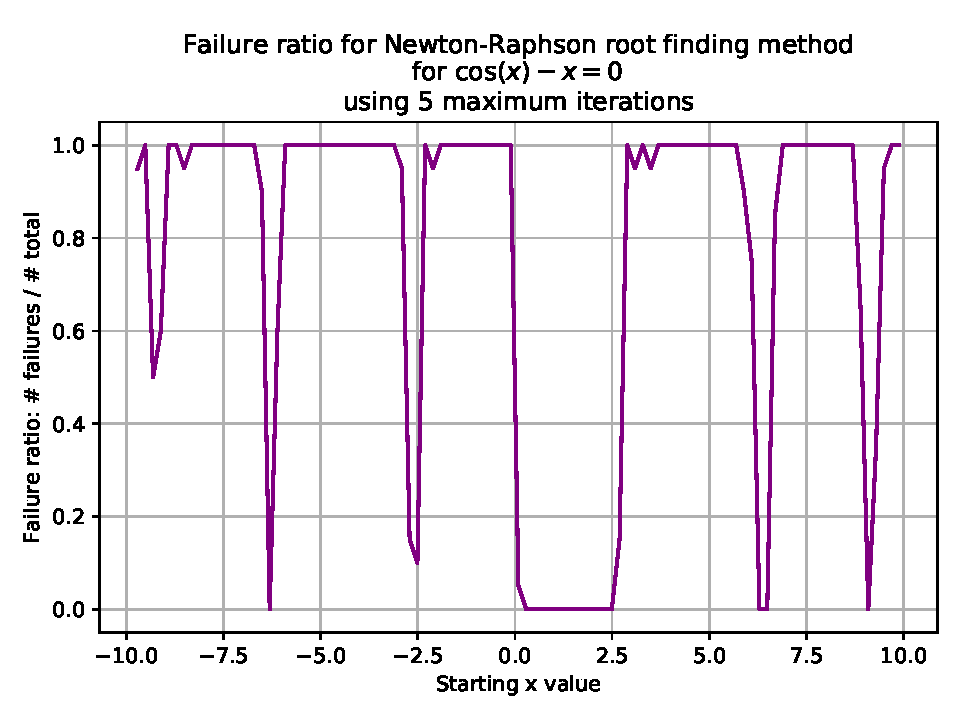
\includegraphics[width=0.8\textwidth]{figures/plot_max_iterations_5.pdf}
  \caption{Failure ratio of Newton-Raphson root finding method for five maximum number of iterations. Failure ratio is close to zero in the interval $[0, 2.5]$.}
  \label{fig_fail_rates_max_iterations_5}
\end{figure}
Increasing the number of iterations to $50$ has decreased the failure ratio for most values of $x_0$ to $0.6$ and lower (\autoref{fig_fail_rates_max_iterations_50}). However, we can still see that all calculation failed for $x_0$ between about $-1$ and $0$. Another peak in failure rates is visible around $x=5$. This could be cause of the small slope of $f(x)$ around $x=-1$ and $x=5$ (\autoref{fig_cos_x_minus_x}). In \autoref{eq_recurrence} the term $f'(x)$ is in the denominator, and small values of $f'(x)$ may cause overflow, or result in very large values of $x_{x+1}$ that are far away from the true root.
\begin{figure}[H]
  \centering
  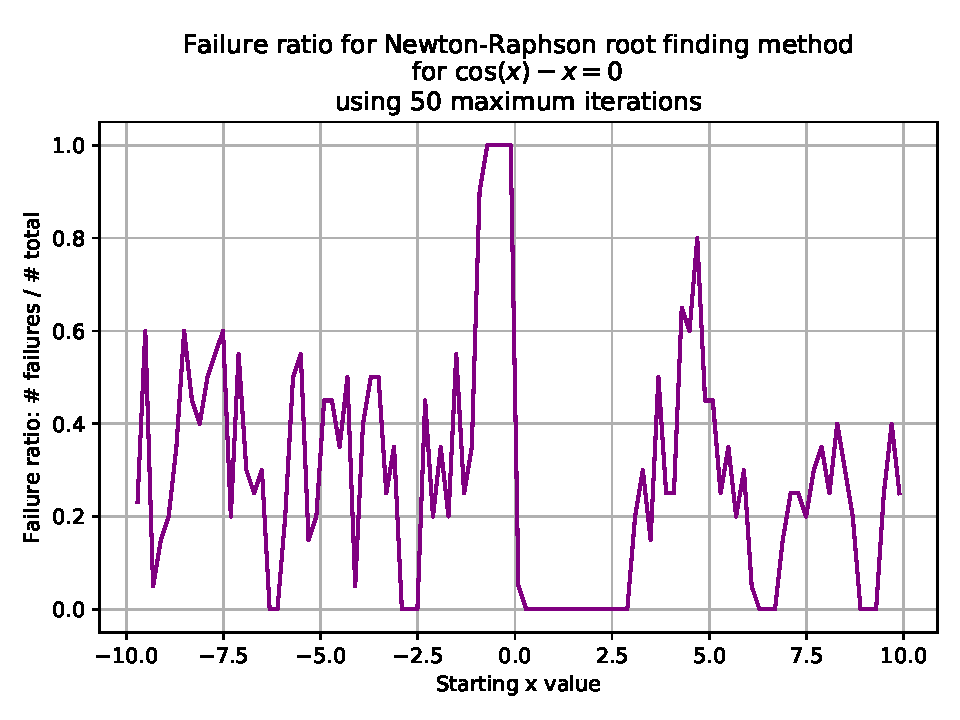
\includegraphics[width=0.8\textwidth]{figures/plot_max_iterations_50.pdf}
  \caption{Failure ratio of Newton-Raphson root finding method for $50$ maximum number of iterations. Failure ratio is close to zero in the interval $[0, 2.5]$}
  \label{fig_fail_rates_max_iterations_50}
\end{figure}
\begin{figure}[H]
  \centering
  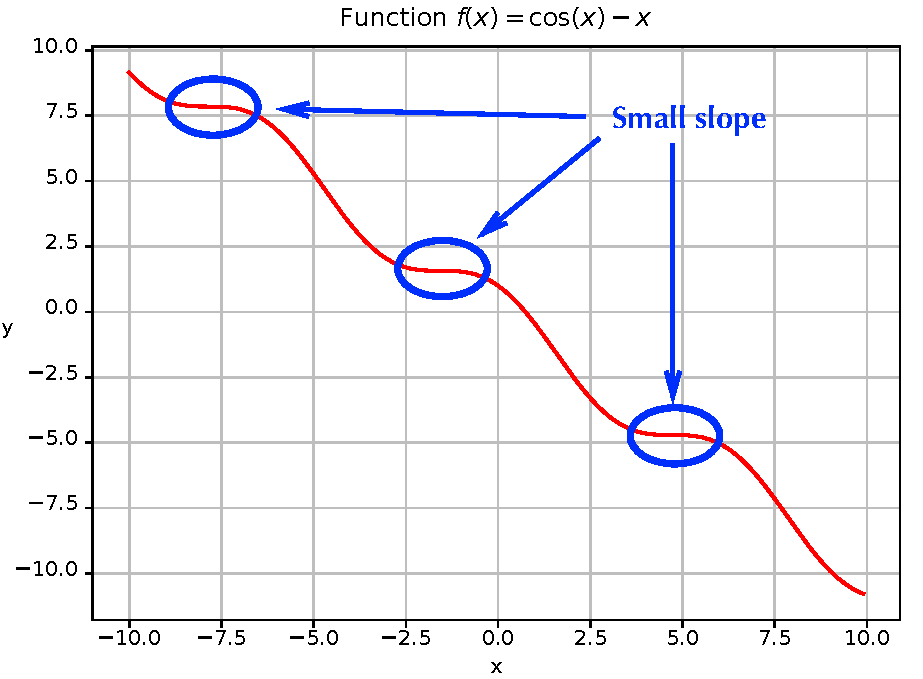
\includegraphics[width=0.8\textwidth]{figures/cos_x_minus_x.pdf}
  \caption{Function $f(x) = \cos(x) - x$.}
  \label{fig_cos_x_minus_x}
\end{figure}
We have found that the failure ratio decreased as we increased $N_{max}$. On \autoref{fig_fail_rates_max_iterations_100000} we can see the failure rate below $0.1$ for most values of $x_0$ when we used very large number of maximum iterations ($N_{max}=\num{100000}$). Interestingly, almost all calculations were still failing for $x_0 \in [-1, 0]$, while values of $x_0$ from the other two regions of small slope of $f(x)$ (for $x_0 \approx -7.5$ and $x_0 \approx 5$) had very low failure rates below $0.1$. It is unclear why we saw such a difference in failure rates for regions of $f(x)$ that have same rates of change.
\begin{figure}[H]
  \centering
  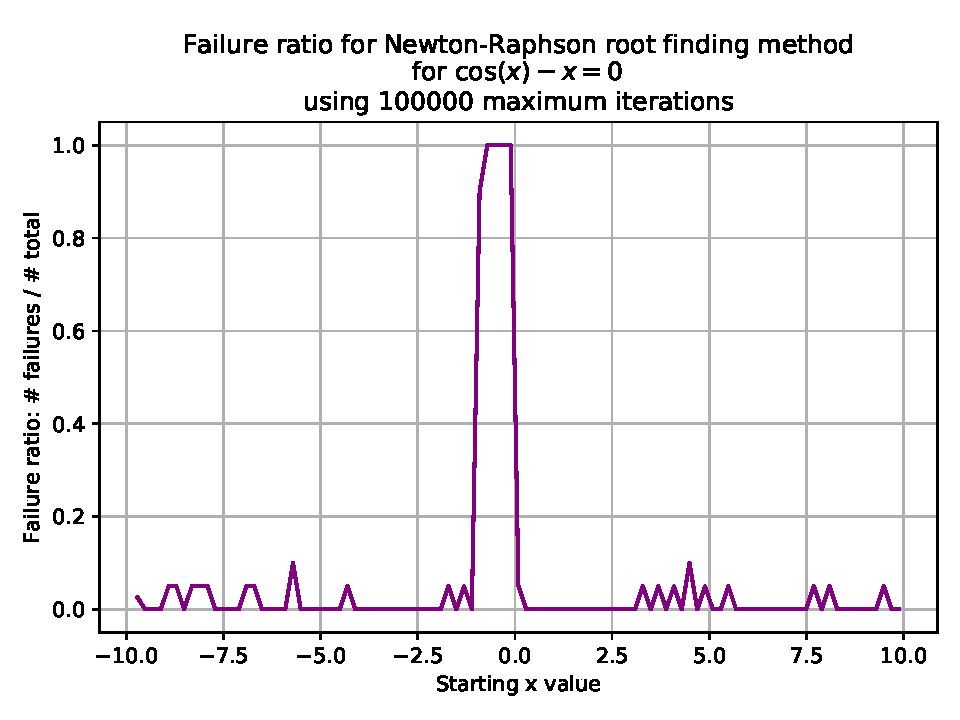
\includegraphics[width=0.8\textwidth]{figures/plot_max_iterations_100000.pdf}
  \caption{Failure ratio of Newton-Raphson root finding method for $\num{100000}$ maximum number of iterations. Failure ratio is close to zero in the interval $[0, 2.5]$}
  \label{fig_fail_rates_max_iterations_100000}
\end{figure}

\section{Failure ratio dependence on $N_{max}$}

Here we investigate how the failure ratio depends on the maximum number of iterations (\autoref{fig_total_failure_ratio}). We can see that the failure ratio is lower with higher $N_{max}$. This is not an unexpected result. When we allow the program to run the calculation from \autoref{eq_recurrence} more times, it might make it more likely for the program to converge.
\begin{figure}[H]
  \centering
  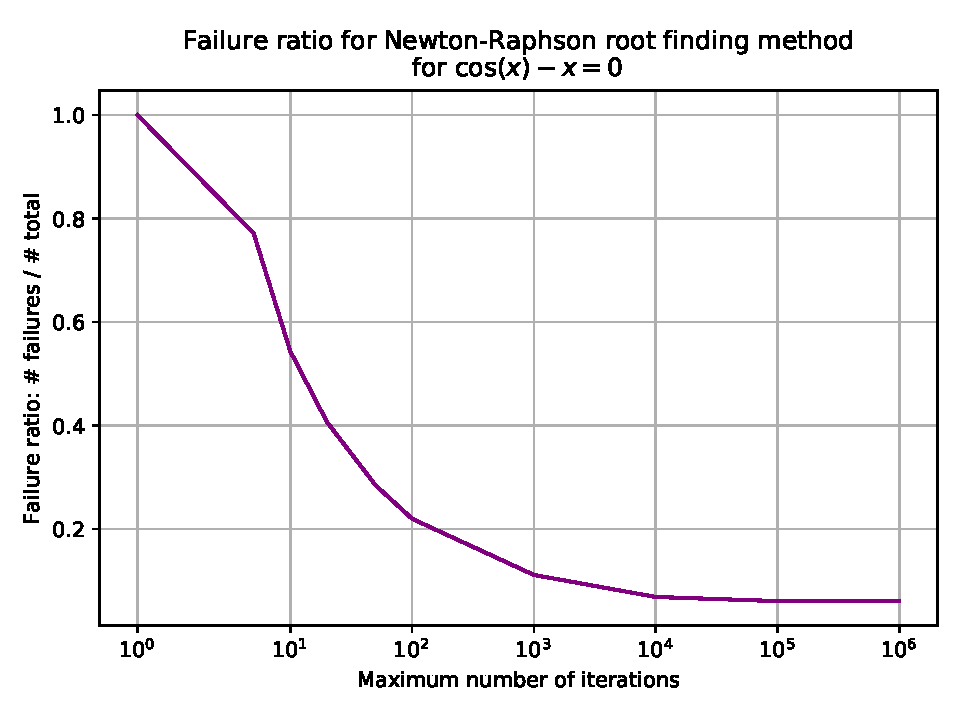
\includegraphics[width=0.8\textwidth]{figures/total_failure_ratio.pdf}
  \caption{Failure ratio of Newton-Raphson root finding method different values of maximum number of iterations.}
  \label{fig_total_failure_ratio}
\end{figure}

\section{Result}

We ran the program with initial value $x_0 = 0.5$, maximum number of iterations $N_{max}=20$ and tolerance $\epsilon=\num{1e-5}$. The program approximated the root to be $0.73909$. Our result agrees with the root calculated by Mathematica code shown in  \autoref{code_find_root_mathematica}.


\noindent\begin{minipage}{\linewidth}
\begin{lstlisting}[caption={Finding root of $\cos(x)-x = 0$ using Mathematica.},frame=tlrb,label={code_find_root_mathematica}]
FindRoot[Cos[x] - x, {x, 0.5}]
{x -> 0.739085}
\end{lstlisting}
\end{minipage}













